\documentclass[a4paper]{article}
\usepackage[lmargin=1cm,rmargin=1cm, top=2cm, bottom=2cm]{geometry}
\usepackage{graphicx}
\usepackage{booktabs}
% \usepackage{multicol}
\usepackage{amssymb}
\usepackage{fancyhdr}
\usepackage{wrapfig}
\usepackage{polynom}
\usepackage{enumitem}
\graphicspath{ {images/} }
\usepackage{lmodern}
\usepackage{amsmath, amsthm, amsfonts}
\usepackage{wasysym}[nointegrals]
\usepackage{relsize}
\usepackage{soul}
\usepackage{listings}
\usepackage{tensor}
\usepackage{pifont}
\usepackage{tikz}
\usepackage{amsfonts}
\usepackage{sectsty}
\usepackage{float}
\usepackage[spanish,es-tabla]{babel}
\usepackage{hyperref}
%\usepackage{caption}
\usepackage{subcaption}
\usepackage{tabularx}
\usepackage{multirow}

\sectionfont{\fontsize{12}{15}\selectfont}
\pagestyle{fancy}
\renewcommand{\headrulewidth}{1pt}
\renewcommand{\footrulewidth}{1pt}
\setlength\headheight{70.0pt}
\addtolength{\textheight}{-35.0pt}

\lhead{
\includegraphics[scale=0.17]{logo.jpg}}
\chead{\emph{Universidad Nacional de Colombia\\Circuitos de RF\\ 	Alejandro Ezequiel Celis Pineda - acelis@unal.edu.co\\ Federik Leonardo Fajardo Useche - felfajardous@unal.edu.co\\Daniel Vega - dvegap@unal.edu.co
\\2024-1}}

\begin{document}
\newpage
\begin{center}
    \Large \textbf{Informe Práctica 5.\\ Mezclador y Oscilador.}
\end{center}

\section{Trabajo previo}
\subsection{Amplificador}
En el diseño del amplificador se selecciona el dispositivo JFET J310 que tiene un rango de frecuencia que incluye los 52MHz.

\subsubsection{Polarización}
\subsubsection{Análisis de estabilidad}
\subsubsection{Simulación}
\subsection{Oscilador}
%\input{Informe/0z0z2Conceptos}
\subsubsection{Diseño}\label{sec:0z0z0Disegno}

\paragraph{Especificaciones}
Se diseñara un oscilador en la banda VHF con una frecuencia de oscilación de 52MHz. 
\paragraph{Polarización}
Se manejará una tensión de 15V cumpliendo con el lineamiento de una fuente con tensión menor o igual a 20v. 
Se escoge primero una corriente de colector de 10mA como una corriente típica para la operación como amplificador de source común para el 2N3904 \cite{alldatasheetcom_2n3904_nodate}. 
Después de esto, se añade una resistencia de emisor para mejorar la estabilidad térmica, colocando así una tensión en el emisor de 1V. 
\begin{equation*}
    R=\frac{1[v]}{5[mA]} \xrightarrow{} 100\Omega
\end{equation*}

Dado que la tensión de emisor es de 1v, se requiere en base una tensión de 1.7v para activar el transistor. Para esto, se diseña un divisor de tensión que tiene en cuenta la corriente de base (recordando que el beta es de 300 aproximadamente y usando la expresión $I_C=\beta I_{\beta}$). Esto resulta en una $I_{\beta}$ de $33\mu A$. Se resuelve que la corriente por el divisor sea de 10 veces la corriente en la base, por lo que se obtiene $330\mu A$ como corriente en el divisor y se calcula la resistencia total del divisor de acuerdo con esto:
\begin{equation*}
    R=\frac{15[v]}{330[\mu A]} \xrightarrow{} 45.5 k\Omega    
\end{equation*}
Ahora, la tensión en base/R2 será de 1.7v, por lo que se requiere que:
\begin{equation*}
    1.7[v]=R_2 \cdot 330 [\mu A] \xrightarrow{} 5.15 k\Omega
\end{equation*}
Por lo que $R_1$ será $40.35k\Omega$.

\paragraph{Amplificador de emisor común}
Se usa la ecuación \ref{eq:GainCommonEmisor} para hallar una ganancia de -1. 
\begin{align*}
    gm&=\frac{I_C}{V_T}=\frac{10mA}{25mV}=0.4\Omega^{-1}
    A_v&=-1=-gm\frac{R_C}{1+gmR_E}=-0.4\frac{R_C}{1+0.4\cdot100}
    R_C&=\frac{1+0.4\cdot 100}{0.4}=102.5
\end{align*}
Como se puede ver, la relación entre la resistencia en el colector y la resistencia en el emisor es prácticamente la que define la ganancia. Por esto, se selecciona una resistencia de $100\Omega$ para el colector, mientras se coloca también un potenciometro en paralelo en el emisor para reducirlo mejorando la relación para tener cierto margen que permita cambiar facilmente la relación como es mostrado en \cite{aaron_danner_colpitts_2023}.  

\paragraph{Circuito tanque Colpitts}
Para lograr que el sistema oscile a la frecuencia de 52MHz, se puede usar la expresión \ref{eq:2} y desarrollarla como se ve en \ref{eq:1}. 

Dado que se busca una ganancia de 1 y los elementos que controlan la ganancia en el circuito tanque son los capacitores ($A=-C_1/C_2$), se escogen los capacitores iguales de 10pF por facilidad, obteniendo una ganancia de -1. Se sabe que la ganancia de este tanque realmente es menor por que los elementos no son puramente reactivos, por lo que la ganancia del bloque de amplificación debe ser mayor.  


\begin{align}
    \label{eq:1}
    \omega &= 2\pi f = \sqrt{\frac{C_1+C_2}{C_1C_2L}} \\
    w &= \sqrt{\frac{2}{CL}} \\
    L &= \frac{2}{C w^2} \\
    L &= \frac{2}{10pF w^2} \\
    L &= 1.87 \mu H
\end{align}

\paragraph{Acople con la carga}
Para el acople con la carga se utiliza el software SIMNec (\cite{SIMNec})


\subsubsection{Simulaciones}\label{sec:0z0z1Simulation}
Se usa Qucs-s para las simulaciones (\cite{noauthor_qucs-s_nodate}). La estrategia es primero simular aparte el circuito amplificador y el circuito tanque, corregir los resultados cambiando valores y estrategias en los dos circuitos y luego unirlos para simular todo el oscilador. 
\paragraph{Amplificador}
En la figura \ref{fig:0z0z1:1} se puede ver la primera simulación teniendo en cuenta la carga de $1M\Omega || 20 pF$. Los valores de resistencia y capacitancia se obtuvieron previamente en la sección \ref{sec:0z0z0Disegno}. Los valores del transistor se obtuvieron del modelo spice de \cite{alldatasheetcom_2n3904_nodate}.

\begin{figure}
    \centering
    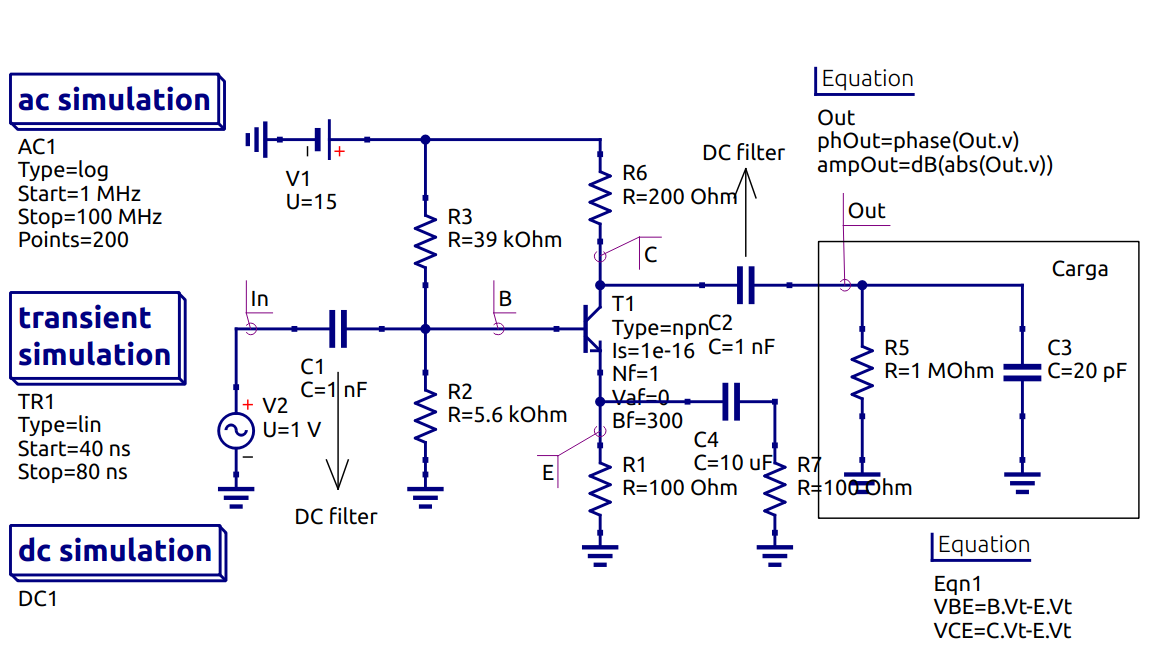
\includegraphics[height=6cm]{Images/13.png}
    \caption{Esquema simulado en \cite{noauthor_qucs-s_nodate} para la sección de amplificación}
    \label{fig:0z0z1:1}
\end{figure}
\begin{figure}
    \centering
    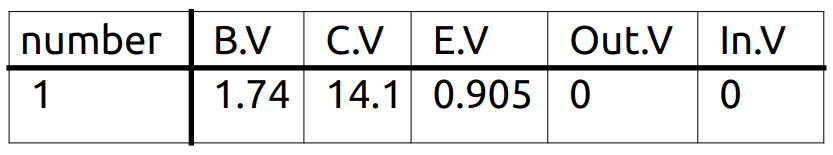
\includegraphics[height=2cm]{Images/5.png}
    \caption{Resultados en DC}
    \label{fig:0z0z1:2}
\end{figure}
La figura \ref{fig:0z0z1:2} se muestran los resultados DC que validan la polarización del transistor 2N3904 \cite{alldatasheetcom_2n3904_nodate}. En la figura \ref{fig:0z0z1:3} se muestran los valores de tensión en la salida del circuito para un rango de frecuencias desde 1 Hz hasta 100MHz. Se puede ver que el comportamiento de filtro de los capacitores efectivamente elimina el componente DC en la salida como se desea. En la figura \ref{fig:0z0z1:3} se hace un zoom a la frecuencia de interés y se ve un comportamiento de filtro pasabajos dado por el capacitor en paralelo de la carga. Sin embargo, se puede ver que existe una amplificación mayor a 0dB, por lo que el diseño aún funciona en el sentido de la magnitud. La fase, sin embargo, tiene que ser corregida con el acople que se implementa más adelante. 

\begin{figure}
    \centering
    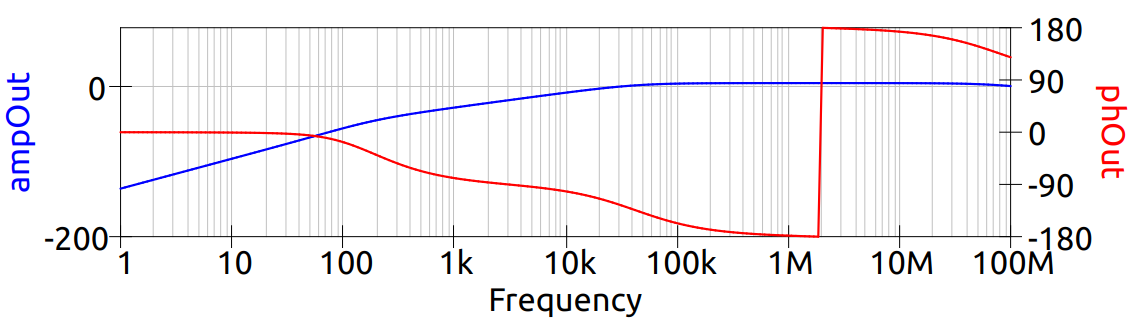
\includegraphics[height=4cm]{Images/16.png}
    \caption{Amplitud y fase de la tensión de salida en dB y grados. Entre 1Hz y 100MHz}
    \label{fig:0z0z1:3}
\end{figure}

\begin{figure}
    \centering
    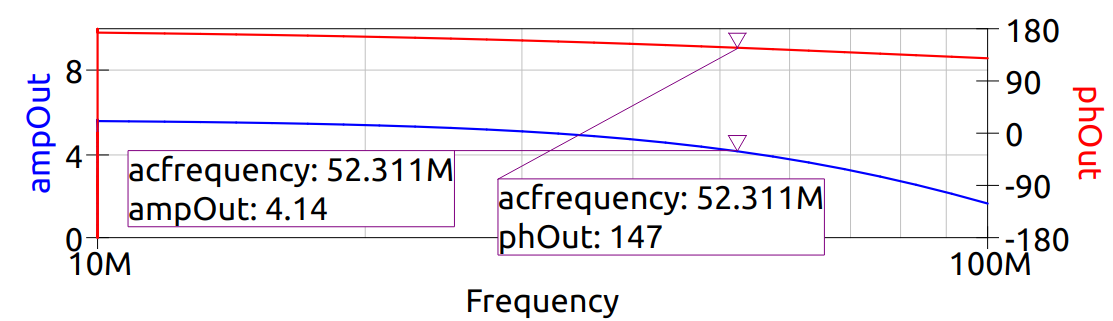
\includegraphics[height=4cm]{Images/17.png}
    \caption{Amplitud y fase de la tensión de salida en dB y grados. Entre 1 MHz y 100MHz}
    \label{fig:0z0z1:4}
\end{figure}



\subsection{Mezclador}
\paragraph{Mezclador}
El mezclador produce la resta y la suma de dos señales entrantes con distintas frecuencias. Si el dispositivo es de recepción, el mezclador normalmente se enfocará en obtener la resta entre la señal de RF y el oscilador local (LO). Si se encuentra en la etapa de transmisión, el mezclador normalmente producirá una señal RF muy superior en frecuencia a la señal de entrada con ayuda de un oscilador local con frecuencia mayor a la frecuencia de entrada IF.
\paragraph{Aislamiento entre puertos}
No se desean los componentes frecuenciales del oscilador local ni de la entrada en la salida o viceversa. Por esta razón los mezcladores al igual que los osciladores pueden ser balanceados o doblemente balanceados. Existen a su vez dos formas principales de implementar estos mezcladores: Mezclador con transistores y mezclador con diodos (y transformadores) En este trabajo se usaron dos mezcladores balanceados (balanceado simple) balanceado usando diodos shotcky 1N4148. 
\subsubsection{Diseño}
Para el diseño se debe considerar si se desea producir una 
\subsubsection{Simulación}
En la siguiente imagen se puede ver el esquema simulado en LTSpice. 
\begin{figure}
    \centering
    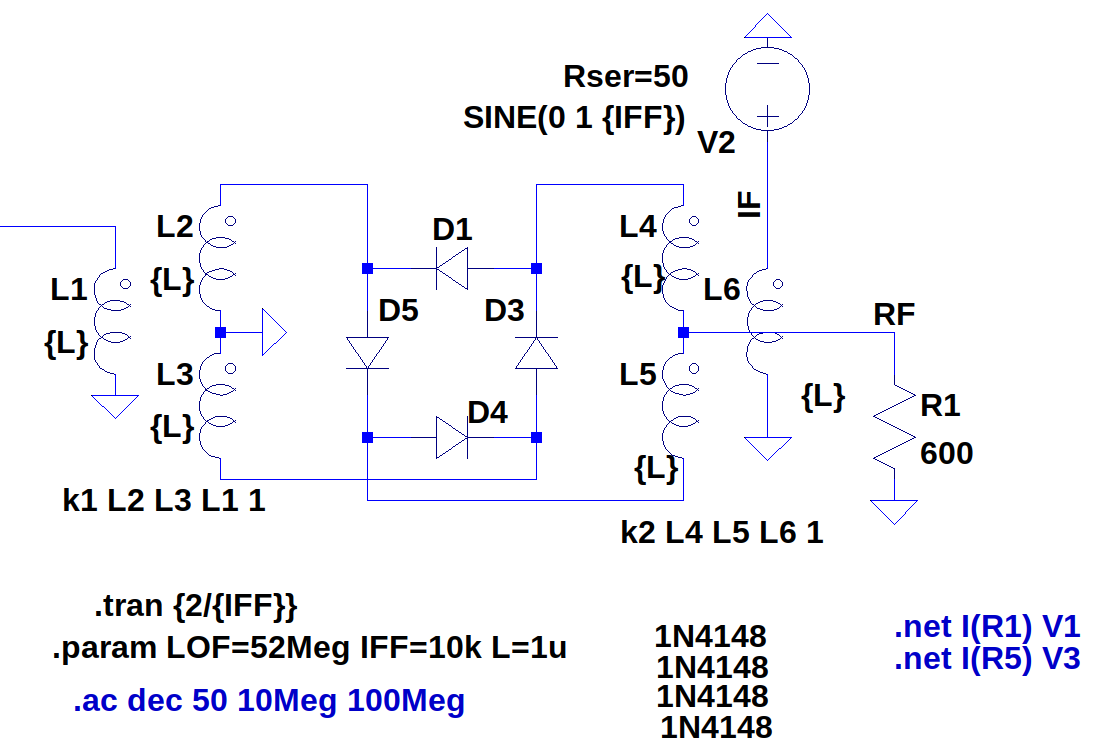
\includegraphics[width=0.5\linewidth]{Images/MIXERSIMU.png}
    \caption{Mezclador de diodos doblemente balanceado}
    \label{fig:mezDiod2}
\end{figure}
\input{Informe/0z0Antena}

%\section{Trabajo previo}
\subsection{Amplificador}
En el diseño del amplificador se selecciona el dispositivo JFET J310 que tiene un rango de frecuencia que incluye los 52MHz.

\subsubsection{Polarización}
\subsubsection{Análisis de estabilidad}
\subsubsection{Simulación}
\subsection{Oscilador}
%\input{Informe/0z0z2Conceptos}
\subsubsection{Diseño}\label{sec:0z0z0Disegno}

\paragraph{Especificaciones}
Se diseñara un oscilador en la banda VHF con una frecuencia de oscilación de 52MHz. 
\paragraph{Polarización}
Se manejará una tensión de 15V cumpliendo con el lineamiento de una fuente con tensión menor o igual a 20v. 
Se escoge primero una corriente de colector de 10mA como una corriente típica para la operación como amplificador de source común para el 2N3904 \cite{alldatasheetcom_2n3904_nodate}. 
Después de esto, se añade una resistencia de emisor para mejorar la estabilidad térmica, colocando así una tensión en el emisor de 1V. 
\begin{equation*}
    R=\frac{1[v]}{5[mA]} \xrightarrow{} 100\Omega
\end{equation*}

Dado que la tensión de emisor es de 1v, se requiere en base una tensión de 1.7v para activar el transistor. Para esto, se diseña un divisor de tensión que tiene en cuenta la corriente de base (recordando que el beta es de 300 aproximadamente y usando la expresión $I_C=\beta I_{\beta}$). Esto resulta en una $I_{\beta}$ de $33\mu A$. Se resuelve que la corriente por el divisor sea de 10 veces la corriente en la base, por lo que se obtiene $330\mu A$ como corriente en el divisor y se calcula la resistencia total del divisor de acuerdo con esto:
\begin{equation*}
    R=\frac{15[v]}{330[\mu A]} \xrightarrow{} 45.5 k\Omega    
\end{equation*}
Ahora, la tensión en base/R2 será de 1.7v, por lo que se requiere que:
\begin{equation*}
    1.7[v]=R_2 \cdot 330 [\mu A] \xrightarrow{} 5.15 k\Omega
\end{equation*}
Por lo que $R_1$ será $40.35k\Omega$.

\paragraph{Amplificador de emisor común}
Se usa la ecuación \ref{eq:GainCommonEmisor} para hallar una ganancia de -1. 
\begin{align*}
    gm&=\frac{I_C}{V_T}=\frac{10mA}{25mV}=0.4\Omega^{-1}
    A_v&=-1=-gm\frac{R_C}{1+gmR_E}=-0.4\frac{R_C}{1+0.4\cdot100}
    R_C&=\frac{1+0.4\cdot 100}{0.4}=102.5
\end{align*}
Como se puede ver, la relación entre la resistencia en el colector y la resistencia en el emisor es prácticamente la que define la ganancia. Por esto, se selecciona una resistencia de $100\Omega$ para el colector, mientras se coloca también un potenciometro en paralelo en el emisor para reducirlo mejorando la relación para tener cierto margen que permita cambiar facilmente la relación como es mostrado en \cite{aaron_danner_colpitts_2023}.  

\paragraph{Circuito tanque Colpitts}
Para lograr que el sistema oscile a la frecuencia de 52MHz, se puede usar la expresión \ref{eq:2} y desarrollarla como se ve en \ref{eq:1}. 

Dado que se busca una ganancia de 1 y los elementos que controlan la ganancia en el circuito tanque son los capacitores ($A=-C_1/C_2$), se escogen los capacitores iguales de 10pF por facilidad, obteniendo una ganancia de -1. Se sabe que la ganancia de este tanque realmente es menor por que los elementos no son puramente reactivos, por lo que la ganancia del bloque de amplificación debe ser mayor.  


\begin{align}
    \label{eq:1}
    \omega &= 2\pi f = \sqrt{\frac{C_1+C_2}{C_1C_2L}} \\
    w &= \sqrt{\frac{2}{CL}} \\
    L &= \frac{2}{C w^2} \\
    L &= \frac{2}{10pF w^2} \\
    L &= 1.87 \mu H
\end{align}

\paragraph{Acople con la carga}
Para el acople con la carga se utiliza el software SIMNec (\cite{SIMNec})


\subsubsection{Simulaciones}\label{sec:0z0z1Simulation}
Se usa Qucs-s para las simulaciones (\cite{noauthor_qucs-s_nodate}). La estrategia es primero simular aparte el circuito amplificador y el circuito tanque, corregir los resultados cambiando valores y estrategias en los dos circuitos y luego unirlos para simular todo el oscilador. 
\paragraph{Amplificador}
En la figura \ref{fig:0z0z1:1} se puede ver la primera simulación teniendo en cuenta la carga de $1M\Omega || 20 pF$. Los valores de resistencia y capacitancia se obtuvieron previamente en la sección \ref{sec:0z0z0Disegno}. Los valores del transistor se obtuvieron del modelo spice de \cite{alldatasheetcom_2n3904_nodate}.

\begin{figure}
    \centering
    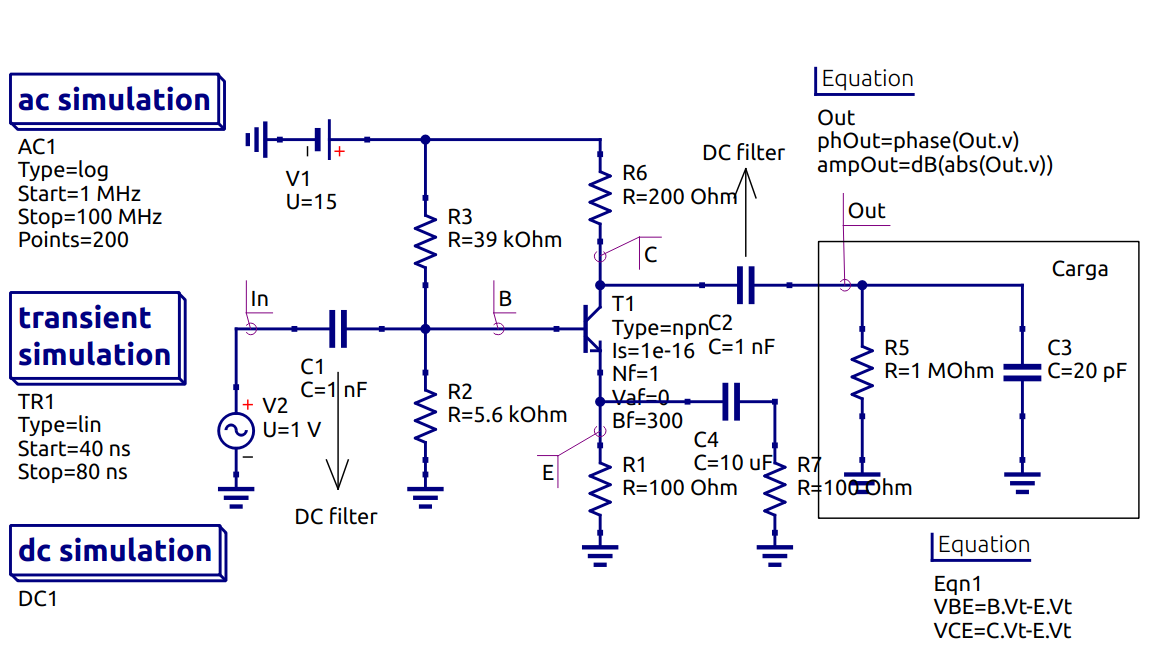
\includegraphics[height=6cm]{Images/13.png}
    \caption{Esquema simulado en \cite{noauthor_qucs-s_nodate} para la sección de amplificación}
    \label{fig:0z0z1:1}
\end{figure}
\begin{figure}
    \centering
    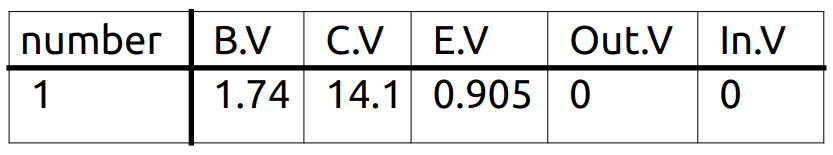
\includegraphics[height=2cm]{Images/5.png}
    \caption{Resultados en DC}
    \label{fig:0z0z1:2}
\end{figure}
La figura \ref{fig:0z0z1:2} se muestran los resultados DC que validan la polarización del transistor 2N3904 \cite{alldatasheetcom_2n3904_nodate}. En la figura \ref{fig:0z0z1:3} se muestran los valores de tensión en la salida del circuito para un rango de frecuencias desde 1 Hz hasta 100MHz. Se puede ver que el comportamiento de filtro de los capacitores efectivamente elimina el componente DC en la salida como se desea. En la figura \ref{fig:0z0z1:3} se hace un zoom a la frecuencia de interés y se ve un comportamiento de filtro pasabajos dado por el capacitor en paralelo de la carga. Sin embargo, se puede ver que existe una amplificación mayor a 0dB, por lo que el diseño aún funciona en el sentido de la magnitud. La fase, sin embargo, tiene que ser corregida con el acople que se implementa más adelante. 

\begin{figure}
    \centering
    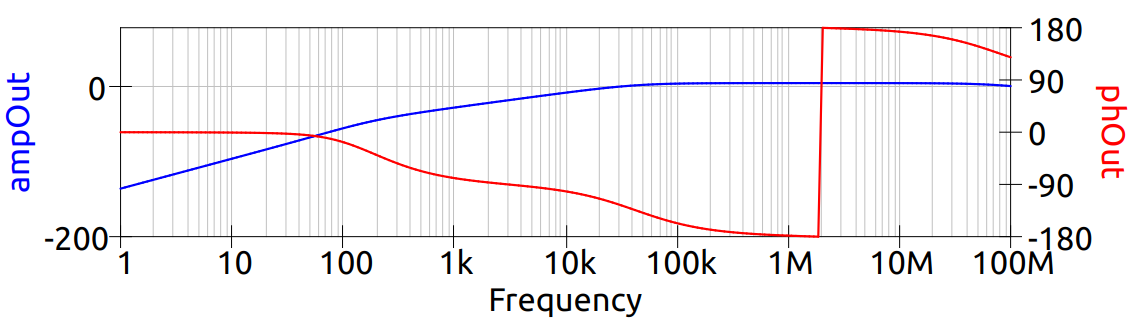
\includegraphics[height=4cm]{Images/16.png}
    \caption{Amplitud y fase de la tensión de salida en dB y grados. Entre 1Hz y 100MHz}
    \label{fig:0z0z1:3}
\end{figure}

\begin{figure}
    \centering
    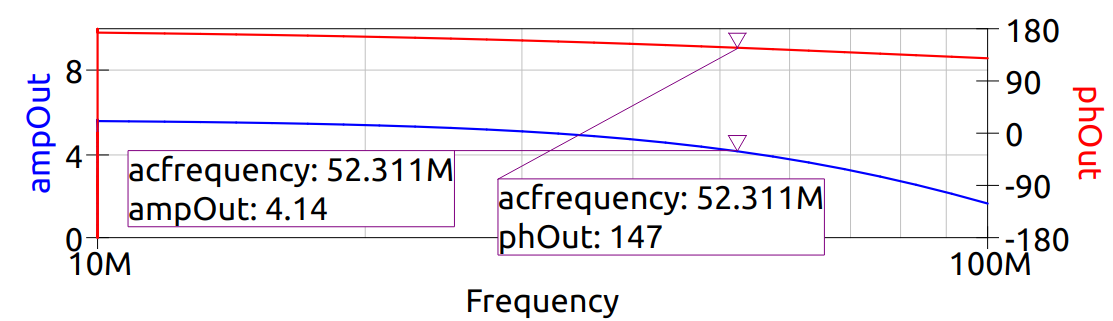
\includegraphics[height=4cm]{Images/17.png}
    \caption{Amplitud y fase de la tensión de salida en dB y grados. Entre 1 MHz y 100MHz}
    \label{fig:0z0z1:4}
\end{figure}



\subsection{Mezclador}
\paragraph{Mezclador}
El mezclador produce la resta y la suma de dos señales entrantes con distintas frecuencias. Si el dispositivo es de recepción, el mezclador normalmente se enfocará en obtener la resta entre la señal de RF y el oscilador local (LO). Si se encuentra en la etapa de transmisión, el mezclador normalmente producirá una señal RF muy superior en frecuencia a la señal de entrada con ayuda de un oscilador local con frecuencia mayor a la frecuencia de entrada IF.
\paragraph{Aislamiento entre puertos}
No se desean los componentes frecuenciales del oscilador local ni de la entrada en la salida o viceversa. Por esta razón los mezcladores al igual que los osciladores pueden ser balanceados o doblemente balanceados. Existen a su vez dos formas principales de implementar estos mezcladores: Mezclador con transistores y mezclador con diodos (y transformadores) En este trabajo se usaron dos mezcladores balanceados (balanceado simple) balanceado usando diodos shotcky 1N4148. 
\subsubsection{Diseño}
Para el diseño se debe considerar si se desea producir una 
\subsubsection{Simulación}
En la siguiente imagen se puede ver el esquema simulado en LTSpice. 
\begin{figure}
    \centering
    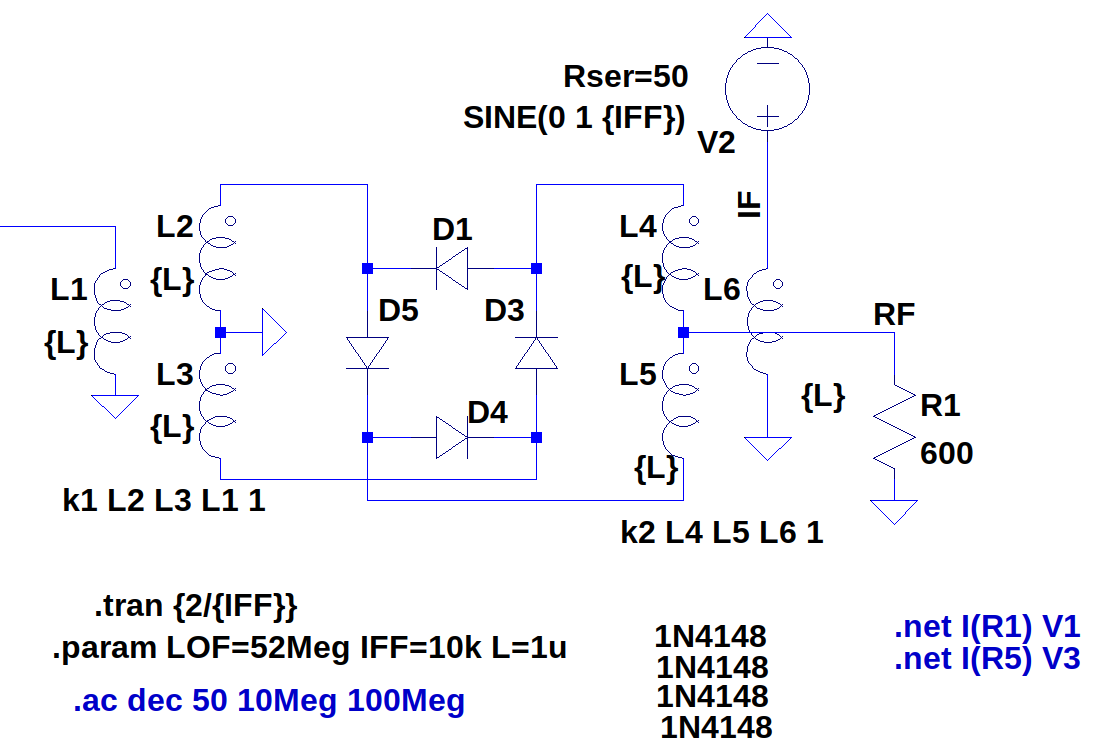
\includegraphics[width=0.5\linewidth]{Images/MIXERSIMU.png}
    \caption{Mezclador de diodos doblemente balanceado}
    \label{fig:mezDiod2}
\end{figure}
\input{Informe/0z0Antena}

%\input{Informe/1Lab}
%\input{Informe/2Posterior}
%\input{Informe/3Conclusiones}

\bibliographystyle{ieeeBibliographyStyle}
\bibliography{refs.bib}
\end{document}
